\section{Experiments and Discussion}

In this section, we report the results of the experiments conducted to test the
efficiency of our algorithms. The experiments test two
queries on difference sizes of machine-generated XML documents, 
ranging from 669 MB to 8 GB.



\subsection{Experimental Data}

The experimental data we used in our experiments is generated by xmlgen, which is an 
XML document generator developed under the an XML benchmark project,  XMark\cite{XMark}. The XMark project aims to provide a benchmark suite that allows users and developers 
to gain insights into the characteristics of their XML repositories. 
It produces XML documents modeling an auction website, a typical e-commerce application. 
The xmlgen-generated data is well-formed, valid, and meaningful to the size of several 
GBytes. The number and type of elements are chosen in accordance with a template and parameterized
 with certain probability distributions. The characteristics of the document are fully preserved under scaling, 
 aiding the analysis of bottlenecks and how they evolve with increasing data volume.

The xmlgen generates XML documents by repeating nodes many times 
from a model tree, which means we can obtain the tree with 
the same structure when nodes that have the same tag names on the 
same level are removed. This root and first level of this model is 
shown in Fig.~\ref{fig:xmlgen1}. The root \texttt{site} has many nodes with different names 
(actually, there are 7 children). The xmlgen generates XML documents of different sizes with only one 
input parameter. For example, we can create 1 GB of file by a parameter of 9.  
In our experiments, the sizes of XML files created by xmlgen range from 
669 MB (the parameter is 7) to 8 GB (the parameter is 72).

\begin{figure} 
	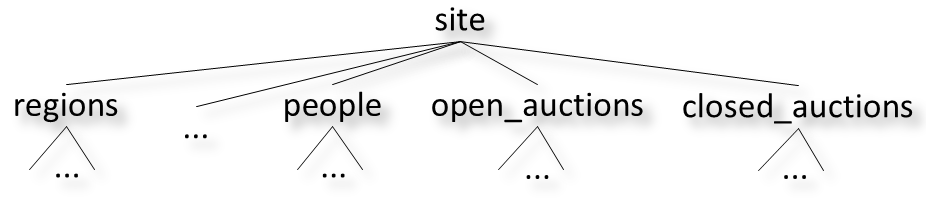
\includegraphics[width=.99\linewidth]{partialtree/figures/xmlgen1.png}
	\caption{Structure of xmlgen generated XML tree}
	\label{fig:xmlgen1}
\end{figure}


To show the effectiveness of our parallel XPath query algorithm, we
perform two types of tests. In the first test, we applied queries to an XML file of 669 MB
to show the scalability of the algorithm with respect to the number of PCs.
In the second test, we fixed the number of PCs to 16 and increased the size of the XML documents.

\begin{table*}[t]
	\caption{Queries used for the experiments}
	\label{table:queries}
	\centering
	\begin{tabular}{c|l}
		\hline
		Q4 & \texttt{/child::site/descendant::keyword/parent::text}\\
		Q5 & \texttt{/child::site/child::people/child::person[child::profile/} \\
		& \texttt{child::gender]/child::name}\\
		Q6 & \texttt{/child::site/child::open\_auctions/child::open\_auction/} \\
		& \texttt{child::bidder[following-sibling::bidder]}\\
		Q7 & \texttt{/child::site/child::closed\_auctions/child::closed\_auction/}\\
		   & \hfill\texttt{child::annotation/child::description/child::text/child::keyword}\\
		\hline
	\end{tabular}
\end{table*}


We use the queries in Table~\ref{table:queries} for our tests.  The
first three queries Q4, Q5, and Q6 test the scalability and
data processing ability.  The last Q7, which has the most steps, is to
test how much the network communications affect the performance.


\subsection{Hardware}

The algorithm was implemented under a server/client architecture 
programmed in Java. The server ran on a single PC, 
which has an Intel(R) Core(TM) i5-760 CPU @ 2.80 GHz CPU, 8 GB of memory, 
and the OS and Java environment are Windows 7 and Java 1.8. 
The clients ran on at most 16 PCs in a PC cluster, where 
9 PCs have Intel(R) Core(TM) i5-2500 @ 3.30 GHz CPU, 7 PCs have Intel(R) have Core(TM) 
i5 CPU 760 @ 2.80GHz, 8 GB of memory, and the OS and Java environment are Ubuntu 14.04 LTS (Linux kernel: 3.16.0-41-generic) and Java 1.8.  
We solely focus on the performance of our algorithms querying on partial trees; 
thus, we construct only one partial tree for each client computer  
and do not use any multi-thread techniques, hyper threading, or other 
memory-sharing techniques. 



\subsection{Parallel speedups}
\label{sec:speedup}

This first experiment tested the efficiency and parallel speedups of
querying with respect to the number of PCs. We use an XML file of size
669 MB and the three queries Q4, Q5, and Q6 with 1, 2, 4, 8 and 16
client PCs. 
The size of XML data on one single computer we have tested is 669 MB. 
We split the input trees evenly by size.

\begin{figure*}[t]
	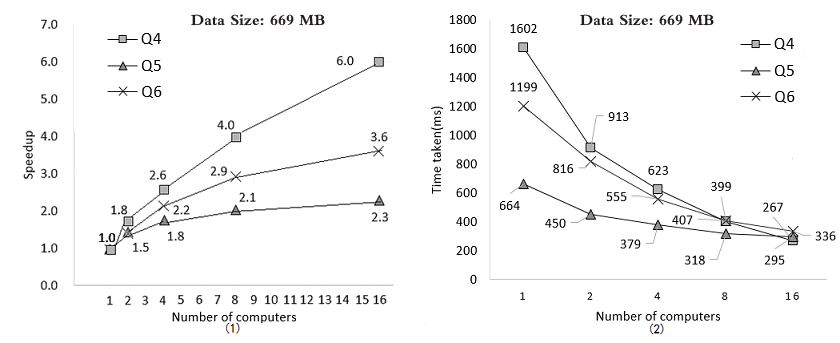
\includegraphics[width=.95\linewidth]{partialtree/figures/ex1.png}
	\caption{Speedups and time with respect to the number of clients PCs}
	\label{fig:exp-1}
\end{figure*}

Fig.~\ref{fig:exp-1} shows the speedups and time taken for the three queries.
The time taken is significantly reduced for all three queries as the number of 
clients increases.
It is more apparent for Q4. Because Q4 has no predicate and the communication affects
the overall time less. We achieved speedups of a factor of 6.0 for Q4 with 16 clients.
Both Q5 and Q6 have a predicate, and it requires more communication phases. 
The speedups for them are relatively low, a factor of 3.6 for Q6 and 2.3 for Q5.
We will discuss these lower speedups by analyzing the network communication cost in Section~\ref{sec:networkcost}.

\subsection{Scalability}
\label{sec:Scalability}

The second experiment is designed to evaluate the performance of data
processing ability per computer as the sizes of input XML data
increase. The size of XML data on a single computer that can be
processed is limited to around 669 MB because of the limit of the size of memory of a
single computer. Some necessary fields and variables of a single node
are declared, which takes extra space that is more than the size of the original XML
string. We split input data at a maximum of 512 MB for a single computer. 
We use 16 computes for
computation, and the sizes of the input XML data range from 1 GB to
8 GB. The time taken is shown in Fig.~\ref{fig:exp-2}~(1).

\begin{figure*}[t]
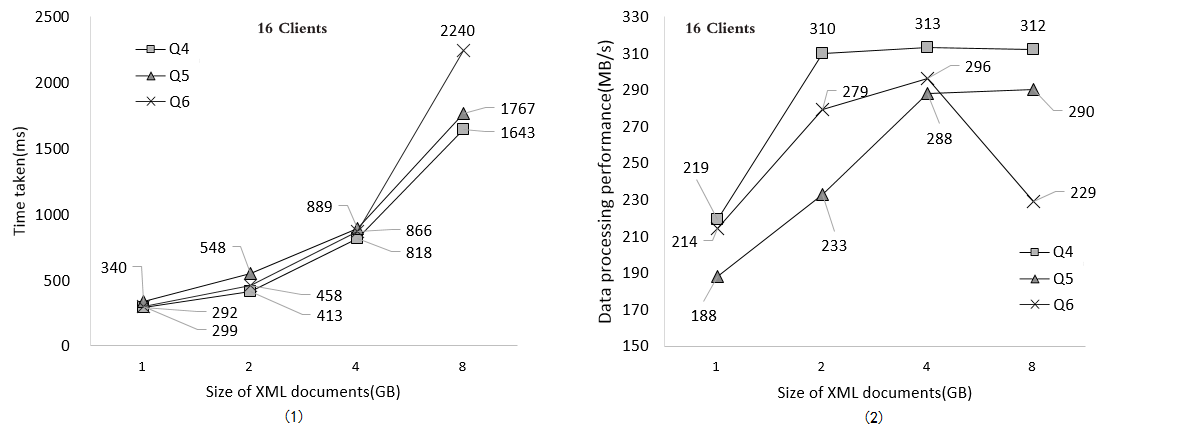
\includegraphics[width=.95\linewidth]{partialtree/figures/ex2.png}
\caption{Time taken and data processing ability}
\label{fig:exp-2}
\end{figure*}
 
The times taken of Q4 and Q5 are almost doubled as the sizes of the input XML
data doubled as shown in Fig.~\ref{fig:exp-2}~(1). For Q6, the time taken is doubled
when the size of data increases from 1 GB to 2 GB and 2 GB to 4 GB. However,
when the size of data increases from 4 GB to 8 GB, the time taken is a little
more than doubled. We believe that the extra time is likely caused by 
the cost by the rapid increase of intermediate
data and the cost of network communication. We will discuss the cost of
the network communication in the following section.

From Fig.~\ref{fig:exp-2}~(2), the data processing ability of a single
computer ranges from about 200 MB/s to 300 MB/s. We also find that when
the size of data increases, the data processing ability increases as
well. It also attributes to the cost of the network communication.



\subsection{Communication Cost}
\label{sec:networkcost}

Our algorithms are implemented with server/client architecture. 
The communication between the server and the clients is based
on TCP/IP protocol. The server is in charge of partial tree construction and 
evaluation control of queries. It holds the information of open nodes of all the partial trees,
including the ranges. The communication mechanism in our framework is based on string messages. 
We tested the communication between the server and the clients. The results
are shown in Fig.~\ref{fig:exp-3}.
 
\begin{figure*}[t]
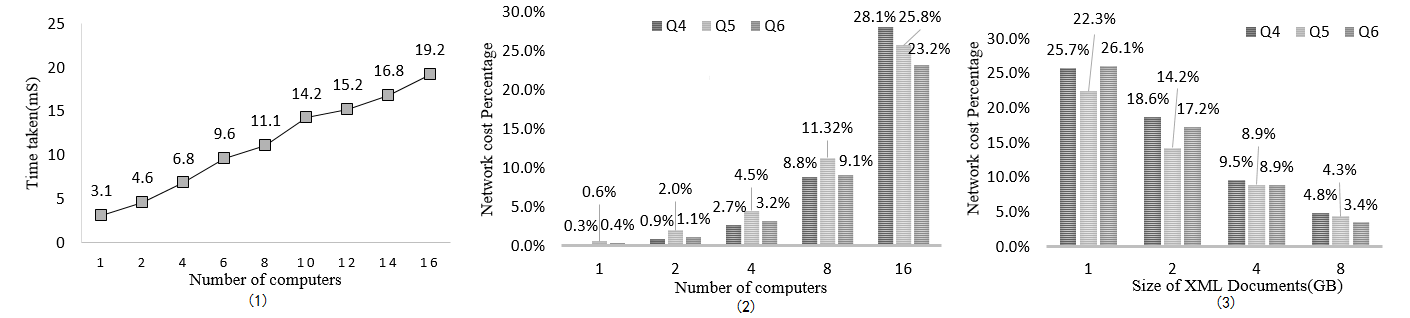
\includegraphics[width=.95\linewidth]{partialtree/figures/ex3.png}
\caption{Cost of network communication}
\label{fig:exp-3}
\end{figure*}

As we can see in Fig.~\ref{fig:exp-3}~(1), when a new client is added,
it takes approximately 1 extra millisecond for a single step on the network. 
For 16 clients, each query step takes around 20 ms for network
communication. We also tested Q7. Even if we use more computers, we obtain a
speedup of less than 1, which means the efficiency is slowed down by the
cost of network communication.

For Q7, the efficiency goes down even when the number of clients
increases. The reason is that for each step of the Q7, it takes around
20 ms for the communication when 16 clients are used. In addition, the
child axis does not take too much time for evaluation. Therefore, the
time saved by increasing the number of clients is wasted due to the cost of
network communication.

We also evaluated the cost of network communication for the former two
experiments. 
For the experiments in Section~\ref{sec:speedup}, as we can
see in Fig.~\ref{fig:exp-3}~(2), the more computers are used, the more
time is taken on network communication.  That is why the speedup increase 
was not obvious when more computers were added.  We can obtain the
same conclusion from Fig.~\ref{fig:exp-3}~(3).  

For the experiments in this section, since the number of computers are the same,
the time taken on network is almost the same. When the size of the
data increases, the effect of network communication becomes
less. Therefore, we can conclude that we can obtain better performance as
the size of the data increases. For the network, if we could improve the 
implementation to reduce the cost of network communication, 
we could get better performance for a small amount of data.

\subsection{Imbalance of Xmlgen-generated XML tree}
After analyzing these data carefully, we find that our 
algorithm does not show the best performance by using these XML documents,
because of the imbalanced structure of xmlgen-generated XML documents. 

In Fig.~\ref{fig:xmlgen1}, the children of the root have different tags. 
When we evaluate an XPath query on this tree by using 
our algorithm, we sometimes only query a small part of the tree, which means we apply queries 
on some of the partial trees that contain specific nodes while we do nothing to the others partial trees. 

For example, as we can see in Fig.~\ref{fig:xmlgen2}, the highlighted parts
are the traversed edges of the tree by Q7. We use two computers for the query. 
The specific nodes are all on the first partial tree on computer 1. 
While on computer 0, there is no node that has the tag name "\texttt{close\_auction}" 
as child of \texttt{site}; therefore, computer 1 is idle after testing the second step of Q7. 

From our experiments, we also find that only part of the computers take part in the computation. 
When we use only one computer for loading 669 MB of data, the total number of nodes is 10023967. And there are 
15300 \texttt{person} nodes for Q5 and 72000 \texttt{closed\_auction} nodes for Q6.
As we can see in Table ~\ref{table:discussionexp16} and ~\ref{table:discussionexp4}, 
we only obtain 2 out of PCs 4 and 3 out of 16 PCs that have a result node after
processing \texttt{/child::person} in Q5. That means only a few of the PCs are used in the query while the others are idle. 
We also notice that when the number of computers increased from 4 to 16, 
the us of the computers for computation only increased from 2 to 3 for \texttt{child::people}.
Thus, we cannot utilize the total number of PCs. We can obtain the same 
conclusion when we take a look at the data for processing \texttt{/child::close\_auction} step in Q6. 

One more thing we have noticed is the imbalance of nodes distribution of partial trees. 
Note that for PC$_9$ or PC$_1$$_0$, there are almost three times more nodes compared to others.
Due to the fact that we need to wait until all the computers' work is done for the next step, 
the imbalanced distribution of nodes also reduces the speedup of these experiments. 
 
From the above discussion, we come to the conclusion that the structure 
of input XML documents affects the speedups of the experiments. 
If we apply our algorithm to some well-balanced XML trees, 
we could obtain better speedups related to the increase in the number of computers.


\begin{table}[t]
	\caption{16 PCs are used for steps in Q5 and Q6.}
	\label{table:discussionexp16}
	\centering
	\begin{tabular}{c|c|c|c}
		\hline
		\hline
	 PC id	& Nodes Count	& /person & /open\_auctions \\ 		
		\hline 
		1 &	442240	& 0	& 0  \\ 
		\hline 	
		2 &	444828		& 0	& 0  \\ 
		\hline 	
		3 &	442158		& 0	& 0  \\ 
		\hline 		
		4 &	444515		& 0	& 0  \\ 
		\hline 		
		5 &	441671		& 0	& 0  \\ 
		\hline 		
		6 &	442697		& 0	& 0  \\ 
		\hline 		
		7 &	442021		& 0	& 0  \\ 
		\hline 	
		8 &	546640 &	14247 & 0	\\
		\hline
		9 &	1331617 &	102551 & 0	\\
		\hline
		10 & 1042920	& 36204	& 12032 \\
		\hline
		11 &	886279	&0	& 18666 \\
		\hline
		12 &	890306  & 0 &	18643 \\
		\hline
		13 & 891300		& 0 & 18720 \\
		\hline
		14 &	591080	& 0	& 3943 \\
		\hline
		15 &	513317	& 0 & 0	\\
		\hline
		16 &	230460	& 0 & 0	 \\
		\hline 
	\end{tabular}
\end{table}

\begin{table}[t]
	\caption{4PCs are used for steps in Q5 and Q6}
	\label{table:discussionexp4}
	\centering
	\begin{tabular}{c|c|c|c}
		\hline
		\hline
		PC id	& Nodes Count	& /person & /open\_auctions \\ 		
		\hline 
		1 &	1773703	& 0	& 0  \\ 
		\hline 	
		2 &	1872954		& 14242	& 0  \\ 
		\hline 	
		3 &	4151158		& 138759	& 49338  \\ 
		\hline 		
		4 &	2226168		& 0	& 22663  \\ 
		\hline
	\end{tabular}
\end{table}


\begin{figure}[t]
	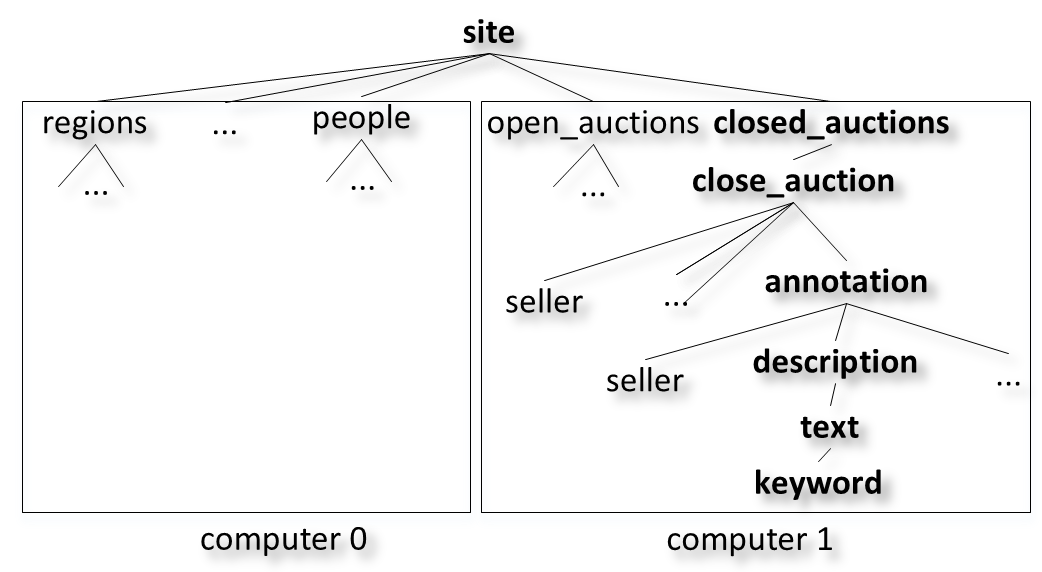
\includegraphics[width=.99\linewidth]{partialtree/figures/xmlgen2.png}
	\caption{An example of tree assignment to computers}
	\label{fig:xmlgen2}
\end{figure}

% LocalWords: kmatsu LTS xmlgen XMark scalability TCP IP